\documentclass[12pt]{article}
%\usepackage[utf8]{inputenc}
%\documentclass[UTF8]{ctexart}
%\usepackage[UTF8, heading = false, scheme = plain]{ctex}
\usepackage{geometry}
%geometry{a4paper,scale=0.9}
\geometry{a4paper,left=1cm,right=1cm,top=1cm,bottom=2cm}
\usepackage{amsfonts}
\usepackage{color}
\usepackage{url}
%\usepackage{biblatex}
\usepackage{amsmath}
\usepackage{amssymb}
\usepackage{latexsym}
\usepackage{listings}
\usepackage[usenames,dvipsnames]{xcolor}
\usepackage{cite}
%\addbibresource{ref.bib}
%\bibliography{ref.bib}
\usepackage{caption}
\usepackage{graphicx, subfig}
\usepackage{float}
%\usepackage[fontset=ubuntu]{ctex}
%\usepackage{fontspec}
\usepackage{xeCJK}
%\usepackage[colorlinks,
%anchorcolor=black,
%citecolor=black]{hyperref}
%\setmainfont{SimSun}
\usepackage[section]{placeins}
\usepackage{enumitem}
\usepackage{framed}
\usepackage[framemethod=TikZ]{mdframed}
\usepackage{indentfirst}
\usepackage{setspace}%使用间距宏包
\linespread{1.5}
\definecolor{mygreen}{rgb}{0,0.6,0}
\definecolor{mygray}{rgb}{0.5,0.5,0.5}
\definecolor{mybgray}{rgb}{0.95,0.95,0.95}
\definecolor{mymauve}{rgb}{0.58,0,0.82}
\lstset{
 backgroundcolor=\color{mybgray}, 
 basicstyle = \footnotesize,       
 breakatwhitespace = false,        
 breaklines = true,                 
 captionpos = b,                    
 commentstyle = \color{mygreen}\bfseries,
 extendedchars = false,             
 frame =shadowbox, 
 framerule=0.5pt,
 keepspaces=true,
 keywordstyle=\color{blue}\bfseries, % keyword style
 language = C++,                     % the language of code
 otherkeywords={string}, 
 numbers=left, 
 numbersep=5pt,
 numberstyle=\tiny\color{mygray},
 rulecolor=\color{black},         
 showspaces=false,  
 showstringspaces=false, 
 showtabs=false,    
 stepnumber=1,         
 stringstyle=\color{mymauve},        % string literal style
 tabsize=2,          
 title=\lstname                      
}

\title{题目汇总 II}
\author{leolinuxer}
%\date{June 2020}

\begin{document}
%\setlength{\parindent}{0pt}
\maketitle
\tableofcontents

\section{高效寻找素数}
\url{https://github.com/labuladong/fucking-algorithm/blob/master/%E9%AB%98%E9%A2%91%E9%9D%A2%E8%AF%95%E7%B3%BB%E5%88%97/%E6%89%93%E5%8D%B0%E7%B4%A0%E6%95%B0.md}

高效解决这个问题的核心思路是:

首先从 2 开始,我们知道 2 是一个素数,那么 2 × 2 = 4, 3 × 2 = 6, 4 × 2 = 8... 都不可能是素数了。

然后我们发现 3 也是素数,那么 3 × 2 = 6, 3 × 3 = 9, 3 × 4 = 12... 也都不可能是素数了。

看到这里,你是否有点明白这个排除法的逻辑了呢?先看我们的第一版代码:
\begin{lstlisting}
int countPrimes(int n) {
    boolean[] isPrim = new boolean[n];
    // 将数组都初始化为 true
    Arrays.fill(isPrim, true);

    for (int i = 2; i < n; i++) 
        if (isPrim[i]) 
            // i 的倍数不可能是素数了
            for (int j = 2 * i; j < n; j += i) 
                    isPrim[j] = false;
    
    int count = 0;
    for (int i = 2; i < n; i++)
        if (isPrim[i]) count++;
    
    return count;
}
\end{lstlisting}

还有两个细微的地方可以优化:

首先,回想刚才判断一个数是否是素数的 isPrime 函数,由于因子的对称性,其中的 for 循环只需要遍历 [2,sqrt(n)] 就够了。这里也是类似的,我们外层的 for 循环也只需要遍历到 sqrt(n):
\begin{lstlisting}
for (int i = 2; i * i < n; i++) 
    if (isPrim[i]) 
\end{lstlisting}

除此之外,很难注意到内层的 for 循环也可以优化。我们之前的做法是:
\begin{lstlisting}
for (int j = 2 * i; j < n; j += i) 
    isPrim[j] = false;
\end{lstlisting}

这样可以把 i 的整数倍都标记为 false,但是仍然存在计算冗余。

比如 n = 25,i = 4 时算法会标记 4 × 2 = 8,4 × 3 = 12 等等数字,但是这两个数字已经被 i = 2 和 i = 3 的 2 × 4 和 3 × 4 标记了。

我们可以稍微优化一下,让 j 从 i 的平方开始遍历,而不是从 2 * i 开始:
\begin{lstlisting}
for (int j = i * i; j < n; j += i) 
    isPrim[j] = false;
\end{lstlisting}

这样,素数计数的算法就高效实现了,其实这个算法有一个名字,叫做 Sieve of Eratosthenes。看下完整的最终代码:
\begin{lstlisting}
int countPrimes(int n) {
    boolean[] isPrim = new boolean[n];
    Arrays.fill(isPrim, true);
    for (int i = 2; i * i < n; i++) 
        if (isPrim[i]) 
            for (int j = i * i; j < n; j += i) 
                isPrim[j] = false;
    
    int count = 0;
    for (int i = 2; i < n; i++)
        if (isPrim[i]) count++;
    
    return count;
}
\end{lstlisting}

该算法的时间复杂度比较难算,显然时间跟这两个嵌套的 for 循环有关,其操作数应该是:

$n/2 + n/3 + n/5 + n/7 + ... = n \times (1/2 + 1/3 + 1/5 + 1/7...)$

括号中是素数的倒数。其最终结果是 O(N * loglogN),有兴趣的读者可以查一下该算法的时间复杂度证明。

\section{接雨水问题详解}
\url{https://github.com/labuladong/fucking-algorithm/blob/master/%E9%AB%98%E9%A2%91%E9%9D%A2%E8%AF%95%E7%B3%BB%E5%88%97/%E6%8E%A5%E9%9B%A8%E6%B0%B4.md}

先看一下题目:
\begin{figure}[H]
    \centering
    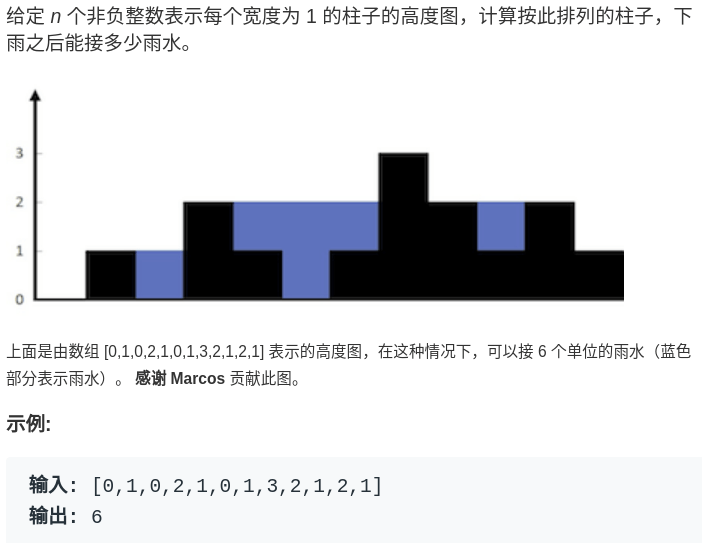
\includegraphics[width=.8\textwidth]{fig/Receive_Rainwater_1.png}
\end{figure}

就是用一个数组表示一个条形图,问你这个条形图最多能接多少水。
\begin{lstlisting}
int trap(int[] height);
\end{lstlisting}

下面就来由浅入深介绍暴力解法 -> 备忘录解法 -> 双指针解法,在 O(N) 时间 O(1) 空间内解决这个问题。

\subsection{核心思路}
我第一次看到这个问题,无计可施,完全没有思路,相信很多朋友跟我一样。所以对于这种问题,我们不要想整体,而应该去想局部;就像之前的文章处理字符串问题,不要考虑如何处理整个字符串,而是去思考应该如何处理每一个字符。

这么一想,可以发现这道题的思路其实很简单。具体来说,仅仅对于位置 i,能装下多少水呢?
\begin{figure}[H]
    \centering
    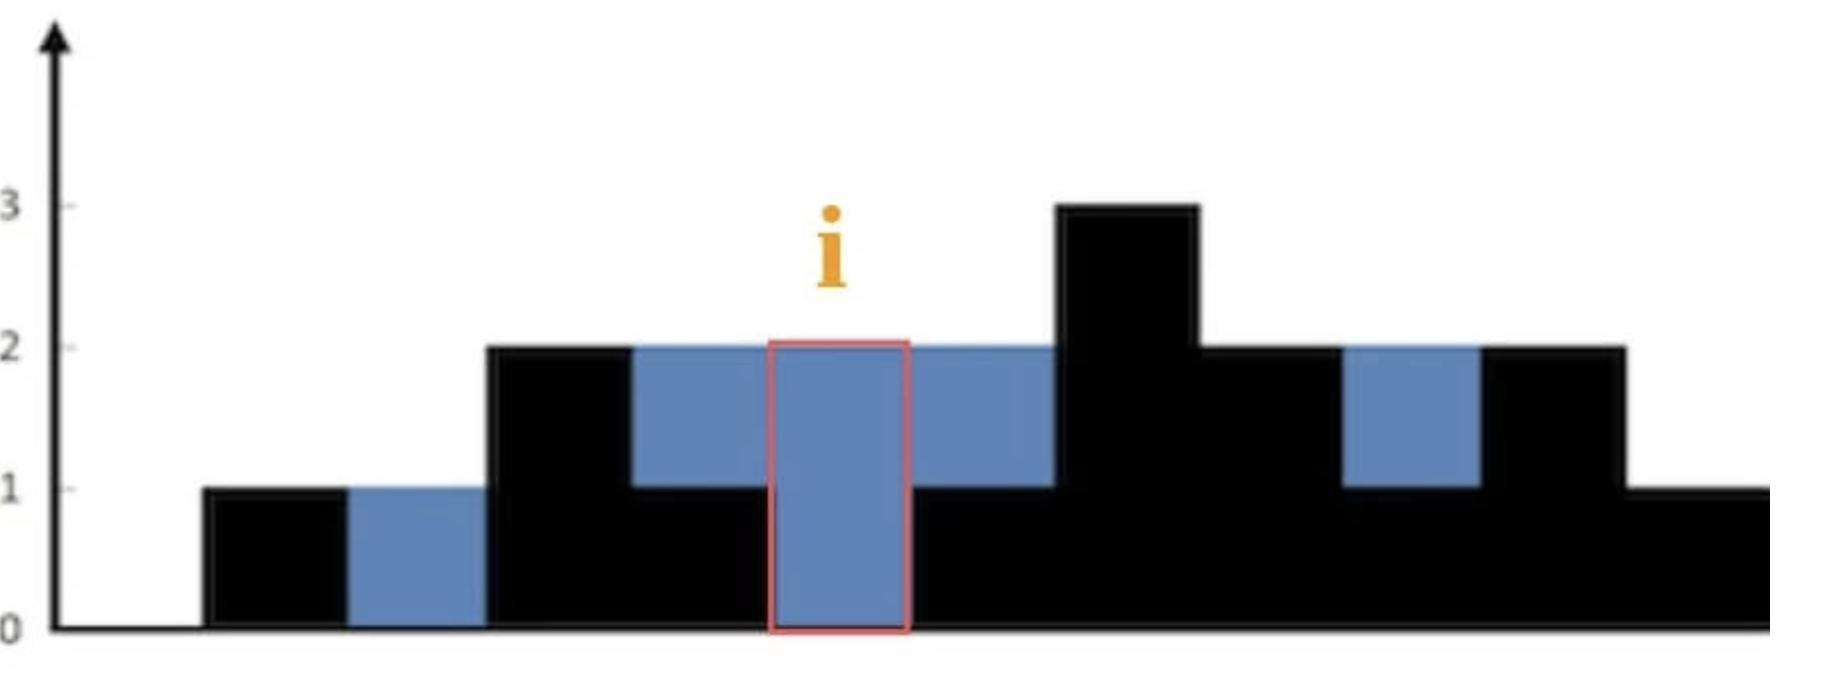
\includegraphics[width=.6\textwidth]{fig/Receive_Rainwater_2.png}
\end{figure}

能装 2 格水。为什么恰好是两格水呢?因为 height[i] 的高度为 0,而这里最多能盛 2 格水,2-0=2。

为什么位置 i 最多能盛 2 格水呢?因为,位置 i 能达到的水柱高度和其左边的最高柱子、右边的最高柱子有关,我们分别称这两个柱子高度为 l\_max 和 r\_max;位置 i 最大的水柱高度就是 min(l\_max, r\_max)。

更进一步,对于位置 i,能够装的水为:
\begin{lstlisting}
water[i] = min(
               # 左边最高的柱子
               max(height[0..i]),  
               # 右边最高的柱子
               max(height[i..end]) 
            ) - height[i]
\end{lstlisting}
\begin{figure}[H]
    \centering
    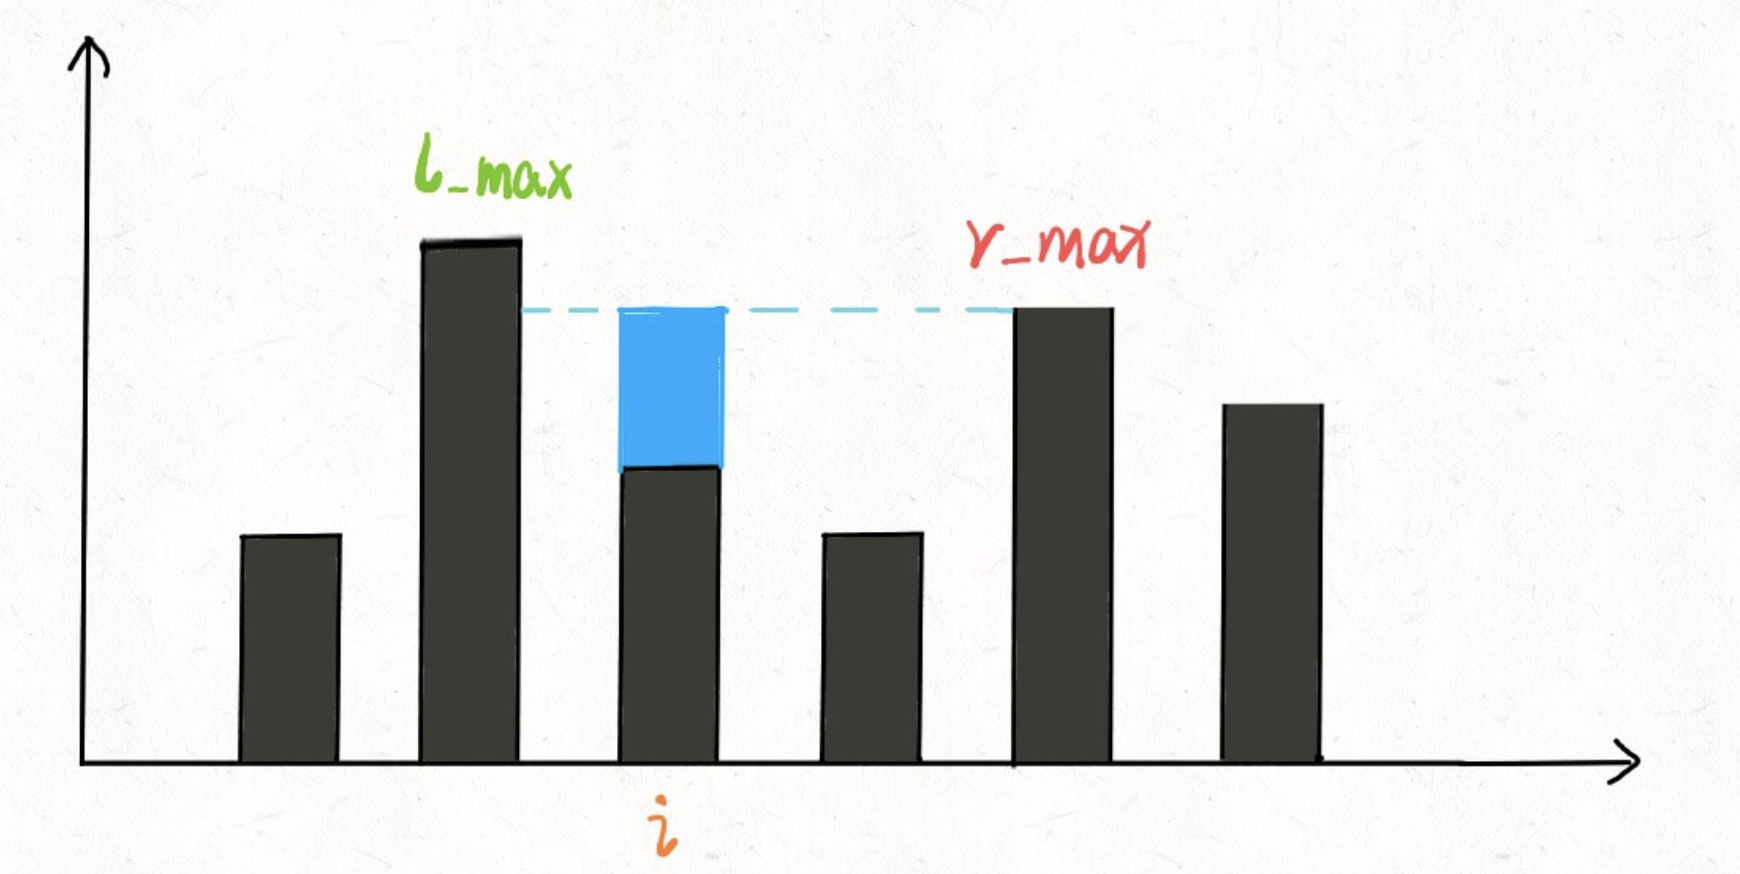
\includegraphics[width=.6\textwidth]{fig/Receive_Rainwater_3.png}
\end{figure}
\begin{figure}[H]
    \centering
    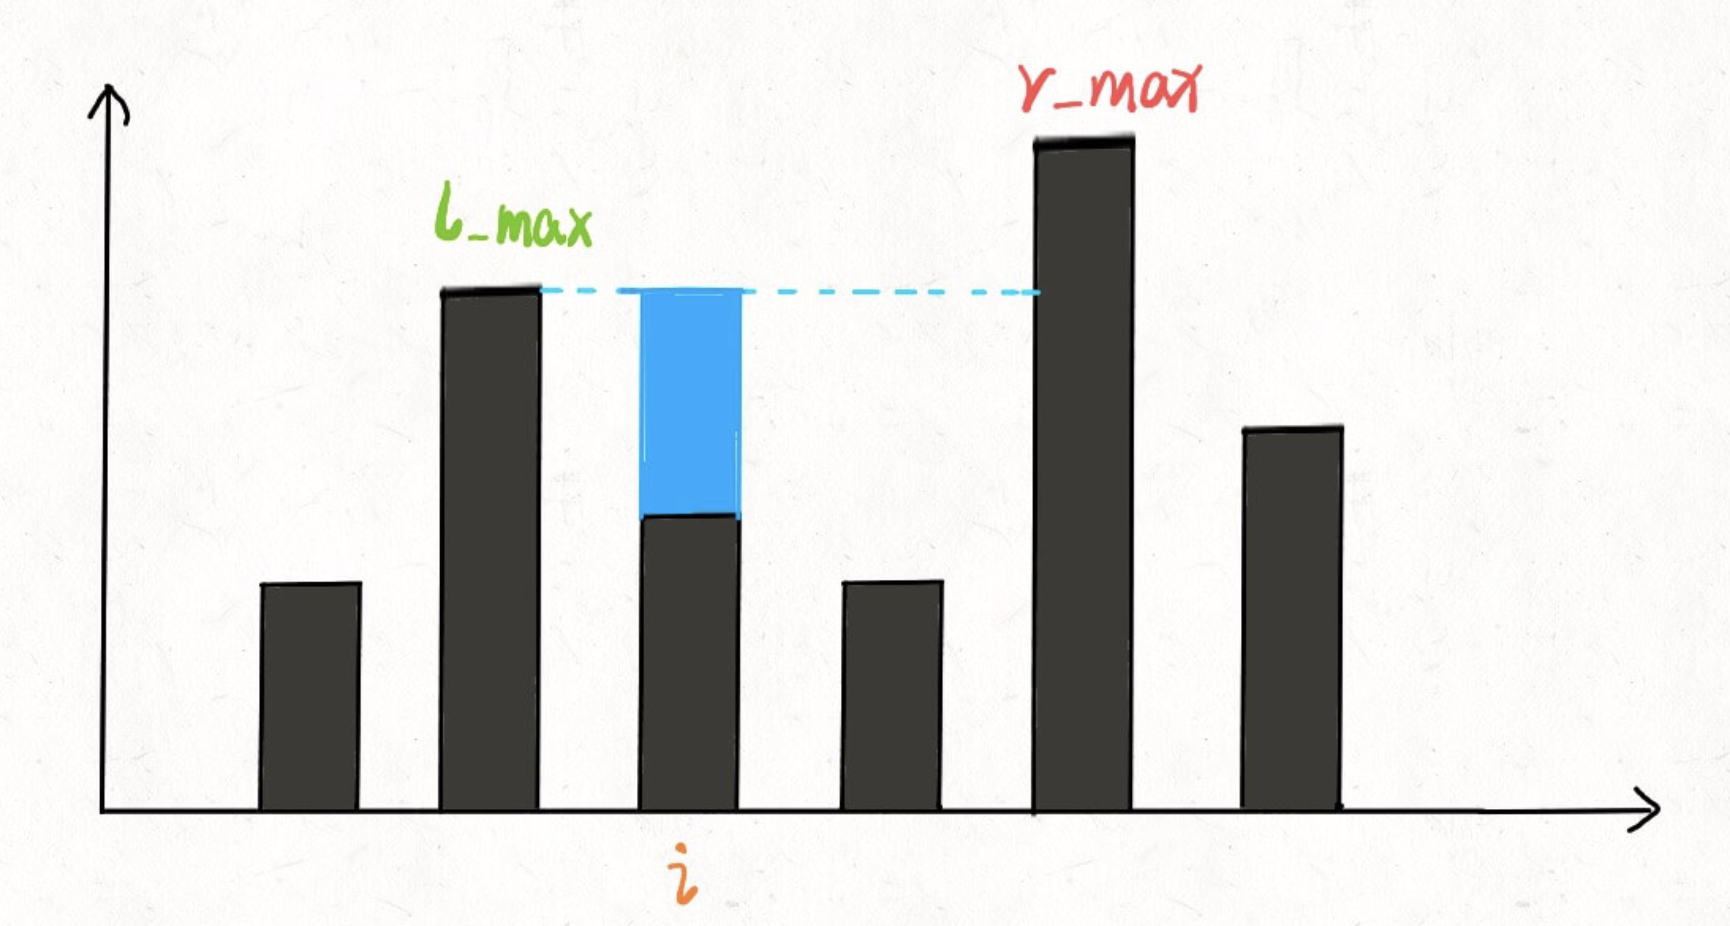
\includegraphics[width=.6\textwidth]{fig/Receive_Rainwater_4.png}
\end{figure}

这就是本问题的核心思路,我们可以简单写一个暴力算法:
\begin{lstlisting}
int trap(vector<int>& height) {
    int n = height.size();
    int ans = 0;
    for (int i = 1; i < n - 1; i++) {
        int l_max = 0, r_max = 0;
        // 找右边最高的柱子
        for (int j = i; j < n; j++)
            r_max = max(r_max, height[j]);
        // 找左边最高的柱子
        for (int j = i; j >= 0; j--)
            l_max = max(l_max, height[j]);
        // 如果自己就是最高的话,
        // l_max == r_max == height[i]
        ans += min(l_max, r_max) - height[i];
    }
    return ans;
}
\end{lstlisting}

有之前的思路,这个解法应该是很直接粗暴的,时间复杂度 $O(N^2)$,空间复杂度 O(1)。但是很明显这种计算 r\_max 和 l\_max 的方式非常笨拙,一般的优化方法就是备忘录。

\subsection{备忘录优化}
之前的暴力解法,不是在每个位置 i 都要计算 r\_max 和 l\_max 吗?我们直接把结果都缓存下来,别傻不拉几的每次都遍历,这时间复杂度不就降下来了嘛。

我们开两个数组 r\_max 和 l\_max 充当备忘录,l\_max[i] 表示位置 i 左边最高的柱子高度,r\_max[i] 表示位置 i 右边最高的柱子高度。预先把这两个数组计算好,避免重复计算:
\begin{lstlisting}
int trap(vector<int>& height) {
    if (height.empty()) return 0;
    int n = height.size();
    int ans = 0;
    // 数组充当备忘录
    vector<int> l_max(n), r_max(n);
    // 初始化 base case
    l_max[0] = height[0];
    r_max[n - 1] = height[n - 1];
    // 从左向右计算 l_max
    for (int i = 1; i < n; i++)
        l_max[i] = max(height[i], l_max[i - 1]);
    // 从右向左计算 r_max
    for (int i = n - 2; i >= 0; i--) 
        r_max[i] = max(height[i], r_max[i + 1]);
    // 计算答案
    for (int i = 1; i < n - 1; i++) 
        ans += min(l_max[i], r_max[i]) - height[i];
    return ans;
}
\end{lstlisting}

这个优化其实和暴力解法差不多,就是避免了重复计算,把时间复杂度降低为 O(N),已经是最优了,但是空间复杂度是 O(N)。下面来看一个精妙一些的解法,能够把空间复杂度降低到 O(1)。

\subsection{双指针解法}
这种解法的思路是完全相同的,但在实现手法上非常巧妙,我们这次也不要用备忘录提前计算了,而是用双指针边走边算,节省下空间复杂度。

首先,看一部分代码:
\begin{lstlisting}
int trap(vector<int>& height) {
    int n = height.size();
    int left = 0, right = n - 1;
    
    int l_max = height[0];
    int r_max = height[n - 1];
    
    while (left <= right) {
        l_max = max(l_max, height[left]);
        r_max = max(r_max, height[right]);
        left++; right--;
    }
}
\end{lstlisting}

对于这部分代码,请问 l\_max 和 r\_max 分别表示什么意义呢?

很容易理解,l\_max 是 height[0..left] 中最高柱子的高度,r\_max 是 height[right..end] 的最高柱子的高度。

明白了这一点,直接看解法:
\begin{lstlisting}
int trap(vector<int>& height) {
    if (height.empty()) return 0;
    int n = height.size();
    int left = 0, right = n - 1;
    int ans = 0;
    
    int l_max = height[0];
    int r_max = height[n - 1];
    
    while (left <= right) {
        l_max = max(l_max, height[left]);
        r_max = max(r_max, height[right]);
        
        // ans += min(l_max, r_max) - height[i]
        if (l_max < r_max) {
            ans += l_max - height[left];
            left++; 
        } else {
            ans += r_max - height[right];
            right--;
        }
    }
    return ans;
}
\end{lstlisting}

你看,其中的核心思想和之前一模一样,换汤不换药。但是细心的读者可能会发现次解法还是有点细节差异:

之前的备忘录解法,l\_max[i] 和 r\_max[i] 代表的是 height[0..i] 和 height[i..end] 的最高柱子高度。

\begin{lstlisting}
ans += min(l_max[i], r_max[i]) - height[i];
\end{lstlisting}
\begin{figure}[H]
    \centering
    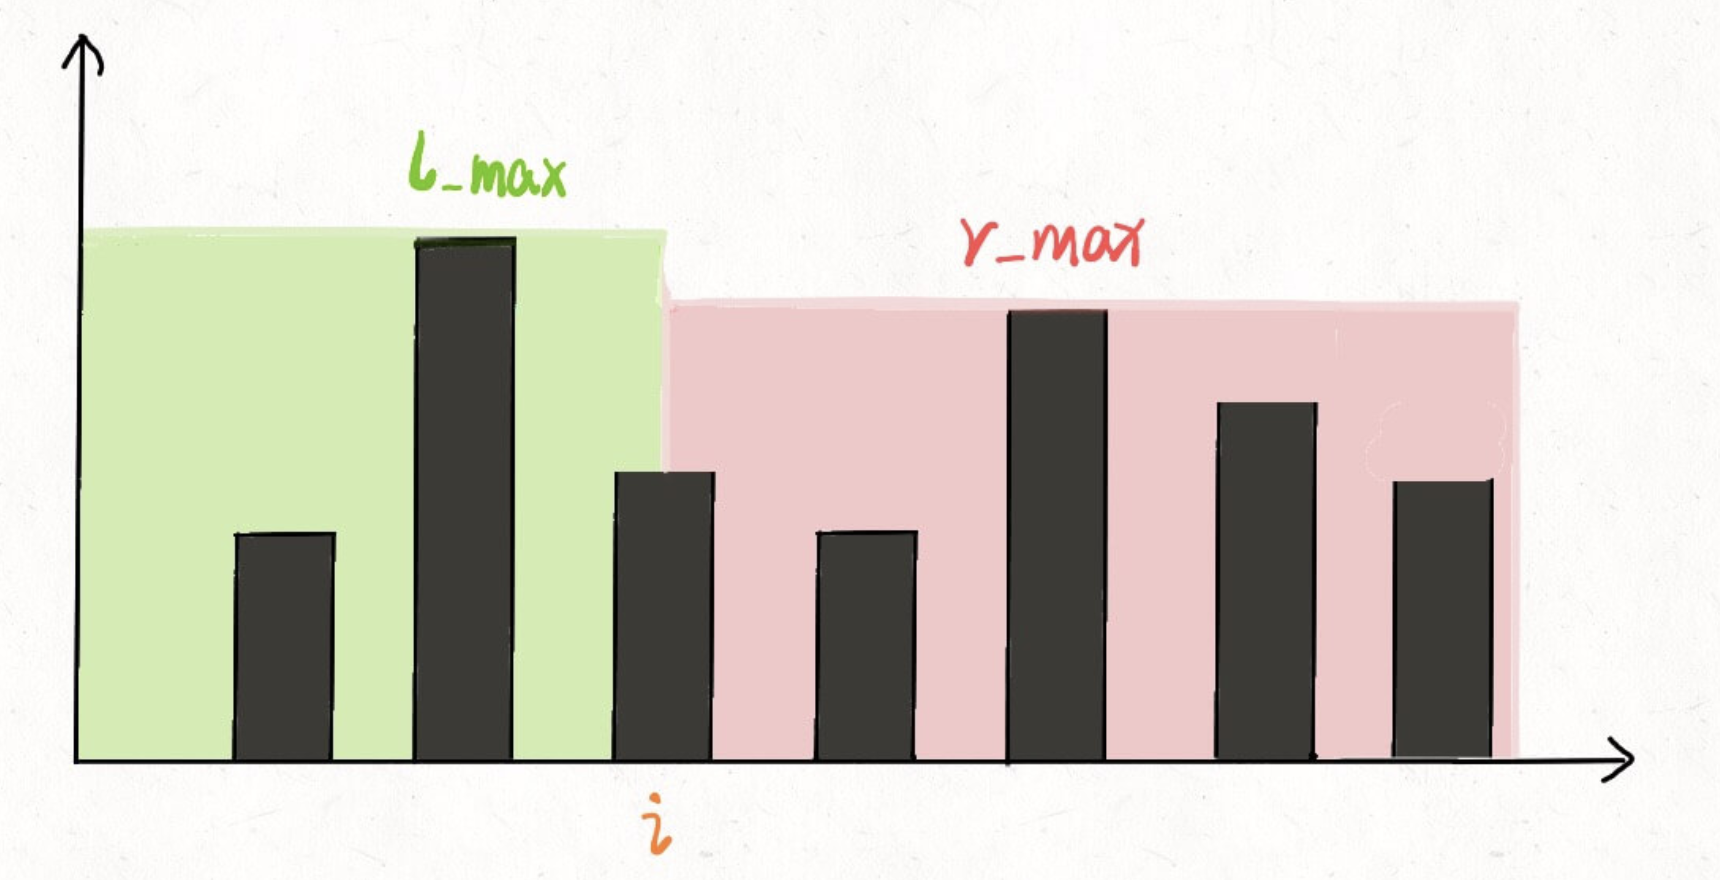
\includegraphics[width=.6\textwidth]{fig/Receive_Rainwater_5.png}
\end{figure}

但是双指针解法中,l\_max 和 r\_max 代表的是 height[0..left] 和 height[right..end] 的最高柱子高度。比如这段代码:
\begin{lstlisting}
if (l_max < r_max) {
    ans += l_max - height[left];
    left++; 
} 
\end{lstlisting}

此时的 l\_max 是 left 指针左边的最高柱子,但是 r\_max 并不一定是 left 指针右边最高的柱子,这真的可以得到正确答案吗?

其实这个问题要这么思考,我们只在乎 min(l\_max, r\_max)。对于上图的情况,我们已经知道 l\_max < r\_max 了,至于这个 r\_max 是不是右边最大的,不重要,重要的是 height[i] 能够装的水只和 l\_max 有关。
\begin{figure}[H]
    \centering
    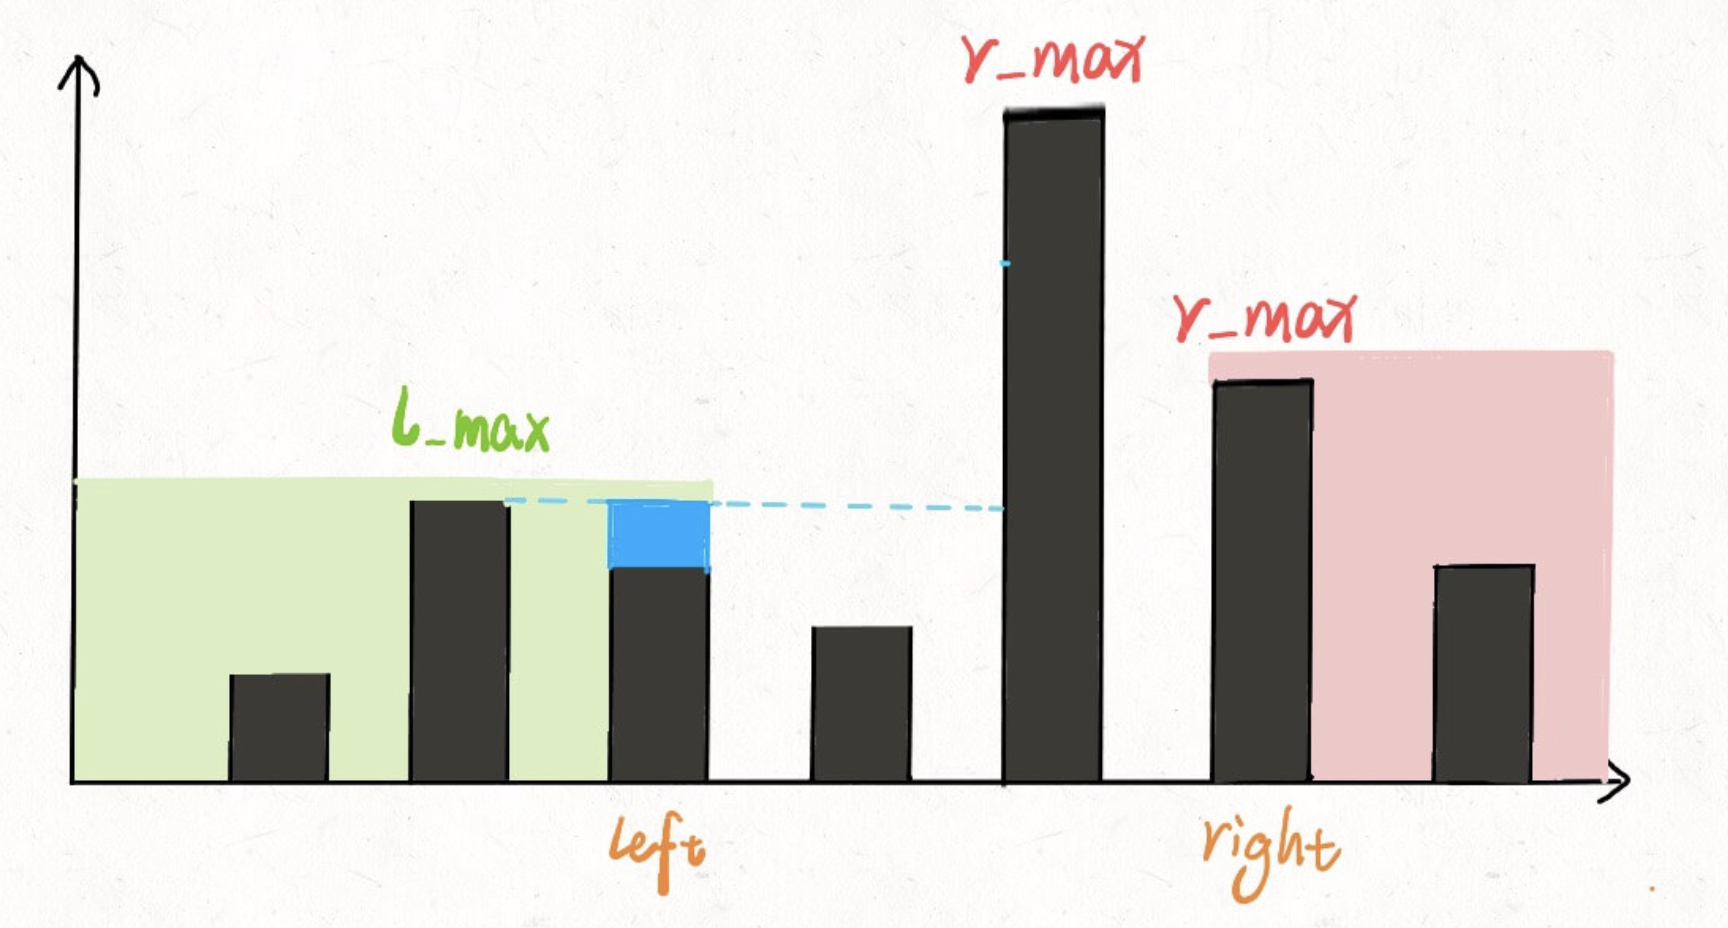
\includegraphics[width=.6\textwidth]{fig/Receive_Rainwater_6.png}
\end{figure}

\section{如何高效进行模幂运算}
\url{https://labuladong.gitbook.io/algo/gao-pin-mian-shi-xi-lie/superpower}

LeetCode 372 题 Super Pow:让你进行巨大的幂运算,然后求余数。
\begin{lstlisting}
int superPow(int a, vector<int>& b);
\end{lstlisting}

要求你的算法返回幂运算 $a^b$计算结果与 1337 取模(mod,也就是余数)后的结果。就是你先得计算幂 $a^b$,但是这个 b 会非常大,所以 b 是用数组的形式表示的。

这个算法其实就是广泛应用于离散数学的模幂算法,至于为什么要对 1337 求模我们不管,单就这道题可以有三个难点:
\begin{itemize}
\setlength{\itemsep}{0pt}
\setlength{\parsep}{0pt}
\setlength{\parskip}{0pt}
    \item \textbf{一是如何处理用数组表示的指数},现在 b 是一个数组,也就是说 b 可以非常大,没办法直接转成整型,否则可能溢出。你怎么把这个数组作为指数,进行运算呢?

    \item \textbf{二是如何得到求模之后的结果}?按道理,起码应该先把幂运算结果算出来,然后做 \% 1337 这个运算。但问题是,指数运算你懂得,真实结果肯定会大得吓人,也就是说,算出来真实结果也没办法表示,早都溢出报错了。
    
    \item \textbf{三是如何高效进行幂运算},进行幂运算也是有算法技巧的,如果你不了解这个算法,后文会讲解。
\end{itemize}

那么对于这几个问题,我们分开思考,逐个击破。

\subsection{如何处理数组指数}
首先明确问题:现在 b 是一个数组,不能表示成整型,而且数组的特点是随机访问,删除最后一个元素比较高效。

不考虑求模的要求,以 b = [1,5,6,4] 来举例,结合指数运算的法则,我们可以发现这样的一个规律:
\begin{align*}
a^{[1,5,6,4]} &= a^4 \times a^{[1,5,6,0]} \\
	&= a^4 \times (a^{[1,5,6]})^{10}
\end{align*}

看到这,我们的老读者肯定已经敏感地意识到了,这就是递归的标志呀!因为问题的规模缩小了:
\begin{lstlisting}
   superPow(a, [1,5,6,4])
=>  superPow(a, [1,5,6])
\end{lstlisting}

那么,发现了这个规律,我们可以先简单翻译出代码框架:
\begin{lstlisting}
// 计算 a 的 k 次方的结果
// 后文我们会手动实现
int mypow(int a, int k);

int superPow(int a, vector<int>& b) {
    // 递归的 base case
    if (b.empty()) return 1;
    // 取出最后一个数
    int last = b.back();
    b.pop_back();
    // 将原问题化简,缩小规模递归求解
    int part1 = mypow(a, last);
    int part2 = mypow(superPow(a, b), 10);
    // 合并出结果
    return part1 * part2;
}
\end{lstlisting}

到这里,应该都不难理解吧!我们已经解决了 b 是一个数组的问题,现在来看看如何处理 mod,避免结果太大而导致的整型溢出。

\subsection{如何处理 mod 运算}
首先明确问题:由于计算机的编码方式,形如 (a * b) \% base 这样的运算,乘法的结果可能导致溢出,我们希望找到一种技巧,能够化简这种表达式,避免溢出同时得到结果。

比如在二分查找中,我们求中点索引时用 (l+r)/2 转化成 l+(r-l)/2,避免溢出的同时得到正确的结果。

那么,说一个关于模运算的技巧吧,毕竟模运算在算法中比较常见:
\begin{lstlisting}
(a * b) % k = (a % k)(b % k) % k
\end{lstlisting}

证明很简单,假设( 其中$A、B、C、D$ 是任意整数),那么:
\begin{align*}
&a \= Ak + B; \ b = Ck + D \\
&\therefore ab = AC*k^2 + AD*k + BC*k + BD \\
&\therefore ab \% k = BD \% k\\
&\because a\%k = B; \ b\%k = D \\
&\therefore (a\%k)(b\%k) \%k = BD \% k = ab \% k
\end{align*}

综上,就可以得到我们化简求模的等式了。

换句话说,\textbf{对乘法的结果求模,等价于先对每个因子都求模,然后对因子相乘的结果再求模}。

那么扩展到这道题,求一个数的幂不就是对这个数连乘么?所以说只要简单扩展刚才的思路,即可给幂运算求模:
\begin{lstlisting}
int base = 1337;
// 计算 a 的 k 次方然后与 base 求模的结果
int mypow(int a, int k) {
    // 对因子求模
    a %= base;
    int res = 1;
    for (int _ = 0; _ < k; _++) {
        // 这里有乘法,是潜在的溢出点
        res *= a;
        // 对乘法结果求模
        res %= base;
    }
    return res;
}

int superPow(int a, vector<int>& b) {
    if (b.empty()) return 1;
    int last = b.back();
    b.pop_back();

    int part1 = mypow(a, last);
    int part2 = mypow(superPow(a, b), 10);
    // 每次乘法都要求模
    return (part1 * part2) % base;
}
\end{lstlisting}

你看,先对因子 a 求模,然后每次都对乘法结果 res 求模,这样可以保证 res *= a 这句代码执行时两个因子都是小于 base 的,也就一定不会造成溢出,同时结果也是正确的。

至此,这个问题就已经完全解决了,已经可以通过 LeetCode 的判题系统了。
但是有的读者可能会问,这个求幂的算法就这么简单吗,直接一个 for 循环累乘就行了?复杂度会不会比较高,有没有更高效地算法呢?

有更高效地算法的,但是单就这道题来说,已经足够了。

因为你想想,调用 mypow 函数传入的 k 最多有多大?k 不过是 b 数组中的一个数,也就是在 0 到 9 之间,所以可以说这里每次调用 mypow 的时间复杂度就是 O(1)。整个算法的时间复杂度是 O(N),N 为 b 的长度。

但是既然说到幂运算了,不妨顺带说一下如何高效计算幂运算吧。

\subsection{如何高效求幂}
快速求幂的算法不止一个,就说一个我们应该掌握的基本思路吧。利用幂运算的性质,我们可以写出这样一个递归式:
$$
a^b = \begin{cases}
a \times a ^{b-1}, \ \text{b为奇数} \\
(a^{b/2})^2, \ \text{b为偶数} \\
\end{cases}
$$

这个思想肯定比直接用 for 循环求幂要高效,因为有机会直接把问题规模(b 的大小)直接减小一半,该算法的复杂度肯定是 log 级了。

那么就可以修改之前的 mypow 函数,翻译这个递归公式,再加上求模的运算:
\begin{lstlisting}
int base = 1337;

int mypow(int a, int k) {
    if (k == 0) return 1;
    a %= base;

    if (k % 2 == 1) {
        // k 是奇数
        return (a * mypow(a, k - 1)) % base;
    } else {
        // k 是偶数
        int sub = mypow(a, k / 2);
        return (sub * sub) % base;
    }
}
\end{lstlisting}


%\printbibliography
\bibliography{../ref}
\bibliographystyle{IEEEtran}
\end{document}